\chapter{Software Requirements}

Requirement identifiers follow the proposal (FR-01 to FR-35, NFR-01 to NFR-10) so that this report, the proposal and the tests refer to the same items. This chapter states the requirements that fall in the Mid scope, with an acceptance check for each; Appendix~B lists all 45 with their Mid status.

\section{User Interactions / Use Cases}

Table~\ref{tab:usecases} lists the use cases that are in scope. The proposal's UC-01 (authenticate), UC-02 (register asset), UC-10 (training), UC-11 (analytics) and UC-12 (manage users) are outside this iteration.

\begin{table}[H]
\centering
\caption{Use cases in scope at FYP-1 Mid}
\label{tab:usecases}
\small
\begin{tabularx}{\textwidth}{@{}c >{\raggedright\arraybackslash}p{0.26\textwidth} >{\raggedright\arraybackslash}p{0.18\textwidth} L@{}}
\toprule
ID & Use case & Primary actor & Entry point in the application \\
\midrule
UC-03 & View aircraft history & Technician & Assets, Asset History, Service Records \\
UC-04 & Upload report & Technician & Ingest (CSV upload, single record) \\
UC-05 & Start diagnosis & Technician & Diagnostics, Quick diagnose \\
UC-06 & Ask follow-up & Technician & Diagnostics, Copilot \\
UC-07 & Inspect evidence & Technician & Evidence links from Diagnostics and the review queue \\
UC-08 & Review conflict & Maintenance supervisor & Review Queue, Detected corrections \\
UC-09 & Explore graph & Technician & Knowledge Graph \\
\bottomrule
\end{tabularx}
\end{table}


\section{Use Case Diagram}

Figure~\ref{fig:usecase} shows the Mid-scope use cases and their primary actors.

\begin{figure}[!htbp]
\centering
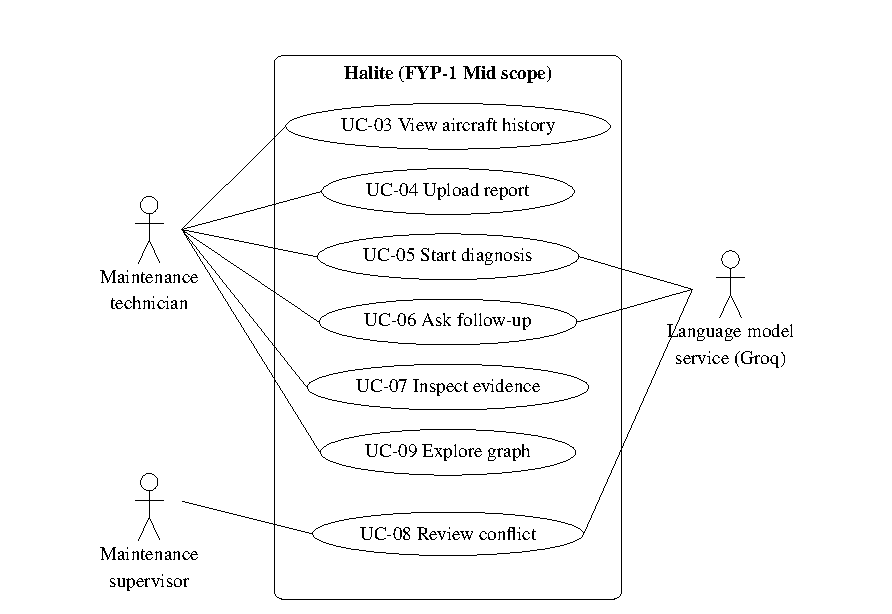
\includegraphics[width=\linewidth,height=0.70\textheight,keepaspectratio]{illustrations/fig_p48_234.pdf}
\caption{Use case diagram. The language model service is a secondary actor: it phrases answers and proposes record classifications, but never decides a ranking. UC-05 and UC-08 both include UC-07: the user can open any cited record from them.}
\label{fig:usecase}
\end{figure}

\section{Detailed Use Cases}

\paragraph{UC-03 View aircraft history.}
Actor: technician. Precondition: records are loaded. Main flow: (1)~The technician opens Assets and sees each aircraft with its record count. (2)~The technician searches by tail number or sorts by record count. (3)~The technician opens an aircraft. (4)~The system shows its records oldest first with the original FAA identifier, component, date and, where present, the analysis result. Alternative: an unknown aircraft shows ``Aircraft not found'', not an empty history. A failed request shows an error with a retry action. Postcondition: nothing is changed.

\paragraph{UC-04 Upload report.}
Actor: technician. Precondition: a CSV in the FAA export format with RegistryNNumber, DifficultyDate (MM/DD/YYYY) and OperatorControlNumber. Main flow: (1)~The technician chooses a \texttt{.csv} file of at most 10~MB; nothing is sent yet. (2)~The technician confirms ``Ingest this file''. (3)~The system stores new records as unanalysed, skips invalid rows and duplicates, and returns counts. (4)~The page shows the counts and a link to the new records. Alternative: a non-CSV or oversize file is rejected before sending; an unreadable file produces an error message; re-uploading the same file reports every record as already stored. Postcondition: new records exist as unscored; existing records are unchanged.

\paragraph{UC-05 Start diagnosis.}
Actor: technician; secondary actor: language model. Precondition: an aircraft with history exists. Main flow: (1)~The technician selects an aircraft and enters a symptom. (2)~The system validates the input and retrieves bounded graph context. (3)~The system ranks inspection checks deterministically. (4)~A live model phrases an explanation from the retrieved records only. (5)~The system verifies every cited record identifier against the graph. (6)~The interface shows the ranked checks, the explanation, the evidence records and the citation status. Alternative~A: no relevant history returns an explicit ``no relevant history'' result without invented records. Alternative~B: no live model returns an HTTP~503 with a reason, and no diagnosis is shown. Alternative~C: an identifier that does not exist is marked unverified. Postcondition: nothing in the graph is changed.

\paragraph{UC-06 Ask follow-up.}
As UC-05, with state carried between turns: the browser holds symptoms, observations, checks done, ruled-out components and open questions, and sends them with each message. The system re-ranks, reports which checks moved up or down, and asks at most one question. If the model is unavailable, the reply is empty but the ranking and evidence are still returned.

\paragraph{UC-07 Inspect evidence.}
Main flow: the technician selects an evidence record identifier; the application opens that record on its aircraft's history page and marks it. Alternative: if the aircraft cannot be resolved, no link is shown and the identifier stays plain text.

\paragraph{UC-08 Review conflict.}
Actor: maintenance supervisor. Precondition: the conflict engine has routed at least one record to review. Main flow: (1)~The supervisor opens the review queue. (2)~The system shows the incoming record beside the retrieved prior record, with the classification, score and rationale. (3)~The supervisor accepts, or rejects with a required note. (4)~The system confirms with the server before changing the screen and stores the status, note and reviewed state. Alternative: an action on a record that is no longer in a reviewable state returns a conflict error and leaves the queue unchanged. Postcondition: the source record is never deleted.

\section{Functional Requirements}

Status key: Met, Partial, Deferred. ``Check'' is the acceptance check.

\subsection{Module M02: Assets}

Table~\ref{tab:fr-m02} lists the Mid-scope asset requirements and their acceptance checks.

\begin{table}[H]
\centering
\caption{Functional requirements --- Assets (M02)}
\label{tab:fr-m02}
\small
\begin{tabularx}{\textwidth}{@{}>{\raggedright\arraybackslash}p{0.10\textwidth} >{\raggedright\arraybackslash}p{0.26\textwidth} L >{\raggedright\arraybackslash}p{0.12\textwidth}@{}}
\toprule
ID & Requirement & Acceptance check & Status \\
\midrule
FR-05 & Register maintenance assets & Assets appear after ingest; no manual registration screen & Partial \\
FR-06 & Display chronological records for an asset & History lists records oldest first; unknown aircraft returns 404 & Met \\
FR-07 & Search assets by identifier & Typing part of a tail number filters the list & Met \\
FR-08 & Display record-linked diagnostic and conflict information & Corrected record shows its corrector; scores and states appear per record & Met \\
\bottomrule
\end{tabularx}
\end{table}

\subsection{Module M03: Knowledge graph}

Table~\ref{tab:fr-m03} lists the Mid-scope knowledge-graph requirements and their acceptance checks.

\begin{table}[H]
\centering
\caption{Functional requirements --- Knowledge graph (M03)}
\label{tab:fr-m03}
\small
\begin{tabularx}{\textwidth}{@{}>{\raggedright\arraybackslash}p{0.10\textwidth} >{\raggedright\arraybackslash}p{0.26\textwidth} L >{\raggedright\arraybackslash}p{0.12\textwidth}@{}}
\toprule
ID & Requirement & Acceptance check & Status \\
\midrule
FR-13 & Create relationships among entities & After ingest every record has ABOUT to its aircraft and PRECEDED\_BY to the earlier record on that aircraft & Met \\
FR-14 & Traverse related historical cases & Graph view shows one aircraft's records and edges; counts equal stored counts & Met \\
FR-15 & Expose provenance of graph results & Legend states which edges come from ingest and which are computed; a record shows its source & Met \\
\bottomrule
\end{tabularx}
\end{table}

\subsection{Module M04: Diagnostics}

Table~\ref{tab:fr-m04} lists the Mid-scope diagnostics requirements and their acceptance checks.

\begin{table}[H]
\centering
\caption{Functional requirements --- Diagnostics (M04)}
\label{tab:fr-m04}
\small
\begin{tabularx}{\textwidth}{@{}>{\raggedright\arraybackslash}p{0.10\textwidth} >{\raggedright\arraybackslash}p{0.24\textwidth} L >{\raggedright\arraybackslash}p{0.14\textwidth}@{}}
\toprule
ID & Requirement & Acceptance check & Status \\
\midrule
FR-16 & Accept natural-language symptoms & Copilot message of 1 to 4000 characters accepted; blank or longer returns 422 & Met \\
FR-17 & Retrieve relevant historical evidence & Context limited to aircraft recent history and fleet scan capped at 2{,}500 records & Met (lexical) \\
FR-18 & Produce ranked hypotheses when evidence suffices & Ranking deterministic: same input gives same order & Met (heuristic) \\
FR-19 & Display supporting record references & Each ranked check lists record identifiers, each a link & Met \\
FR-20 & Ask for clarification when information is missing & Copilot asks at most one question and tracks open questions & Partial \\
FR-21 & Distinguish unsupported from verified & Identifiers absent from the graph marked unverified and omitted from valid list & Met \\
FR-22 & Preserve diagnostic session history & Copilot sessions saved in the browser only; no server-side history & Partial \\
\bottomrule
\end{tabularx}
\end{table}

\subsection{Module M05: Conflict intelligence}

Table~\ref{tab:fr-m05} lists the Mid-scope conflict-intelligence requirements and their acceptance checks.

\begin{table}[H]
\centering
\caption{Functional requirements --- Conflict intelligence (M05)}
\label{tab:fr-m05}
\small
\begin{tabularx}{\textwidth}{@{}>{\raggedright\arraybackslash}p{0.10\textwidth} >{\raggedright\arraybackslash}p{0.24\textwidth} L >{\raggedright\arraybackslash}p{0.14\textwidth}@{}}
\toprule
ID & Requirement & Acceptance check & Status \\
\midrule
FR-23 & Compare new records with prior records & Candidates from same aircraft, earlier in time, with at least one matching signal & Met \\
FR-24 & Classify potential conflicts & Each result is one of five labels; unparseable reply routes to review & Met \\
FR-25 & Route uncertain cases for review & Contradicts and partial\_supersedes always go to review; supersession below 0.50 threshold goes to review & Met \\
FR-26 & Record supervisor decisions & Accept stores status and note; reject requires a non-blank note & Met (no reviewer identity) \\
FR-27 & Audit trail of status changes & Status, review note and state stored; no actor or event log & Partial \\
\bottomrule
\end{tabularx}
\end{table}

\subsection{Module M06: Report intelligence}

Table~\ref{tab:fr-m06} lists the Mid-scope report-intelligence requirements and their acceptance checks.

\begin{table}[H]
\centering
\caption{Functional requirements --- Report intelligence (M06)}
\label{tab:fr-m06}
\small
\begin{tabularx}{\textwidth}{@{}>{\raggedright\arraybackslash}p{0.10\textwidth} >{\raggedright\arraybackslash}p{0.24\textwidth} L >{\raggedright\arraybackslash}p{0.14\textwidth}@{}}
\toprule
ID & Requirement & Acceptance check & Status \\
\midrule
FR-09 & Accept supported report formats & FAA-format CSV by upload or server path, and a single record form & Partial \\
FR-10 & Extract available fields & Tail, date, component, JASC code, location and text stored & Partial \\
FR-11 & Retain the original source record & Text and identifier stored unchanged; reject never deletes & Met \\
FR-12 & Flag ambiguous or invalid fields & Rows with no tail, a bad date or no identifier counted separately & Partial \\
\bottomrule
\end{tabularx}
\end{table}

\section{Non-Functional Requirements}

\subsection{Reliability}

NFR-06: failed external operations are reported and retried safely. Check: a rate-limited model call is retried a bounded number of times; a missing live model returns 503 and never a stored stub as evidence; every page shows a failure state with a retry action and never an empty state that implies ``no data''. Status: met, covered by the backfill, conflict-engine and component tests.

\subsection{Usability}

NFR-08: task completion and a usability score are measured. Status: not measured; no user test was run. Design rules applied instead: errors name the cause, unanalysed records say so, scores carry their meaning, and destructive actions need confirmation.

\subsection{Performance}

NFR-02: non-generation requests meet a p95 of 500~ms. Measured: the assets list took about 0.99~s as a single request on staging, which exceeds the target; no load test was run. The Service Records first load makes two page-initiated requests instead of 119. NFR-03: diagnostic latency is measured under a controlled workload; not measured, because fresh diagnoses call an external model.

\subsection{Security}

NFR-05 (no cross-tenant access) does not apply yet because there is no authentication or tenancy. What exists: the batch analysis and the log-retrieval endpoints need a secret operations token; secrets live in ignored environment files; the settings page no longer offers to wipe the graph. Known risk at the evaluated commit: \texttt{DELETE /api/graph/reset} remained reachable without authentication (Section~8.9); later hardening is noted in Appendix~D.

\section{Acceptance Criteria}

The acceptance criteria are the checks above and the end-to-end acceptance tests T01 to T16 in Chapter~7, which the team defined before the iteration.

\section{Requirements Traceability}

Table~\ref{tab:traceability} traces the central requirements to their design, implementation and tests; the complete matrix is in Appendix~B.

\begin{table}[H]
\centering
\caption{Traceability of central requirements}
\label{tab:traceability}
\small
\begin{tabularx}{\textwidth}{@{}>{\raggedright\arraybackslash}p{0.12\textwidth} L L >{\raggedright\arraybackslash}p{0.22\textwidth}@{}}
\toprule
FR & Design element & Implementation & Tests \\
\midrule
FR-06, 08 & Asset history API and page & \texttt{maintenance.py}, \texttt{AssetHistory.jsx} & \texttt{test\_api\_maintenance}; AssetHistory.test (12) \\
FR-13 & Graph schema, ingest & \texttt{maintenance\_agent.py}, \texttt{queries.py} & \texttt{test\_maintenance\_agent} (10) \\
FR-14, 15 & Graph view & \texttt{Graph.jsx}, \texttt{graphScope.js} & Graph.test (18), graphScope.test (10) \\
FR-17--19 & Retrieval and ranking & \texttt{diagnostic\_retrieval.py} & \texttt{test\_diagnostic\_retrieval} (26) \\
FR-21 & Citation validation & \texttt{citation\_validation.py} & \texttt{test\_citation\_validation} (6) \\
FR-23--25 & Conflict engine & \texttt{conflict\_engine.py} & \texttt{test\_conflict\_engine} (32), cascade (11) \\
FR-26 & Review actions & \texttt{maintenance.py}, \texttt{ReviewQueue.jsx} & ReviewQueue.test (18) \\
FR-09, 12 & CSV upload & \texttt{MaintenanceIngest.jsx} & MaintenanceIngest.test (17) \\
\bottomrule
\end{tabularx}
\end{table}

